\documentclass[]{book}
\usepackage[english]{babel}
\usepackage{graphicx}
\usepackage{amsmath}


\begin{document}


\chapter*{Teoría}

\section{GEM Physics}

% Tal es el caso de los detectores GEM. Tras las generaci´on de pares de electrones
% y iones en el interior de la c´amara de gas por su interacci´on con part´ıculas
% cargadas incidentes, Los electrones libres generados en la ionizaci´on primaria
% son atra´ıdos hacia los agujeros de la hoja de GEM debido al campo el´ectrico.
% Al pasar a trav´es de los agujeros, los electrones experimentan un fuerte campo
% el´ectrico local dentro de estos, lo que causa una avalancha de electrones (multi-
% plicaci´on de electrones), de tal manera que un solo electr´on puede generar varios
% ´ordenes de magnitud de electrones secundarios (ganancia). Los electrones mul-
% tiplicados son recogidos en un conjunto de electrodos o en una segunda capa de
% multiplicaci´on, resultando una se˜nal de corriente el´ectrica que puede ser medida
% y analizada.

\section{Electrónica}

\noindent Como se expuso anteriormente, los electrones multiplicados son recogidos en los electrodos de salida del GEM, resultando una señal de corriente eléctrica que puede ser medida y analizada. Dependiendo de los objetivos del experimento, distintas etapas electrónicas pueden ser implementadas a continuación. Sin embargo, el objetivo de estas converge a preservar y transportar la información física de interés contenida en la señal. \\

\subsection{Electrónica de Front-end}

\noindent Próxima al detector, se encuentra la etapa denominada front-end, que típicamente comprende electrónica analógica para la amplificación de la señal, shaping y discriminación, así como digitalización y transporte. A continuación pueden encontrarse sistemas de más alto nivel como procesadores digitales y de adquisición de datos, que permiten transformar las señales y extraer la información necesaria para su posterior estudio. En la figura \ref{fig:generic_frontend} se observa un esquema genérico de la electrónica de front-end de un detector [1].\\

\begin{figure}[h]
    \centering
    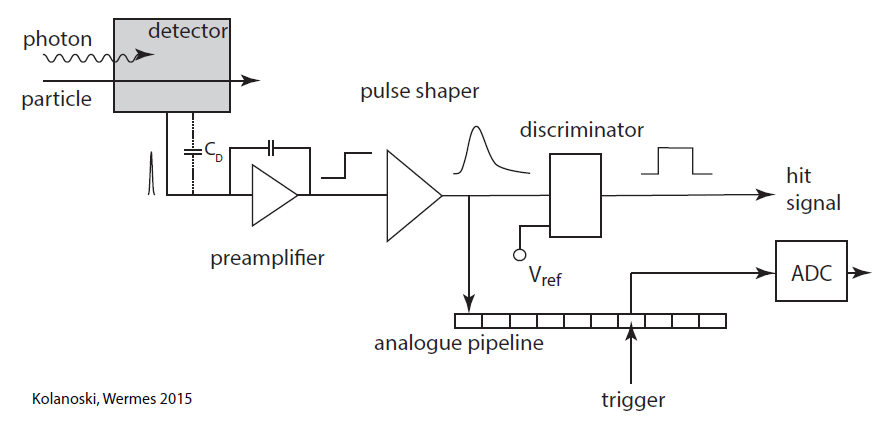
\includegraphics[width=0.7\textwidth]{typical_readout_electronics.PNG}
    \caption{Un esquema de electrónica de front-end típico, utilizado a menudo para la lectura de un
    detector, que incluye amplificación, conformación de impulsos, discriminación
    (aquí analógica) y digitalización (representada aquí por un ADC).}
    \label{fig:generic_frontend}

\end{figure}

\noindent Tal es el caso de los detectores GEM. Las corrientes típicas medidas en su salida pueden ser muy pequeñas, del orden de nanoamperios [citar]. Por lo tanto, es necesario implementar etapas de preamplificación y amplificación, hasta lograr señales con características adecuadas para su digitalización y el subsecuente procesamiento. Sin embargo, la insturmentación típicamente está diseñada para procesar señales de voltaje, por lo que es necesario conectar una resistencia $R$ en serie con la salida del detector para medir una señal de voltaje $V$ en sus terminales, de acuerdo a la ley de Ohm, $$V = R I$$ Como expone [2], La función principal del preamplificador es captar la señal del detector sin deteriorar notablemente la relación señal/ruido inherente. Por ello, el preamplificador se ubica generalmente lo más cerca posible del detector para reducir la carga capacitiva sobre este.\\

\noindent Los sistemas involucrados en la electrónica de front-end, deben cumplir con tres características: (a) ser causales, (b) invariantes en el tiempo, y (c) lineales al menos en la primera etapa de amplificación. Un sistema se considera causal si, en cualquier momento, solo depende del valor de su entrada en ese instante. Es invariante en el tiempo si la relación entre la salida y la entrada, por ejemplo, el ratio señal entrada / señal salida no varía con el tiempo [1]. La linealidad del sistema implica que el pulso de salida (por ejemplo, $v_{out(t)}$) no depende del tamaño de la señal de entrada (por ejemplo, $i_{in(t)}$), esto es, 

$$
v_{\text {out }}\left(\alpha \times i_{\text {in }}(t)\right)=\alpha \times v_{\text {out }}\left(i_{\text {in }}(t)\right)
$$

\noindent Como explica [3], la amplificación por etapas de una señal ofrece numerosas ventajas significativas. Principalmente, permite reducir el ruido generado en cada etapa individual, resultando en una señal final más limpia y menos propensa a la distorsión. Este método también mejora la estabilidad del sistema al distribuir la amplificación, evitando la saturación que podría ocurrir con una amplificación intensa en una sola etapa. Además, facilita el control preciso de la ganancia y la adaptación de impedancias entre diferentes componentes, lo cual mejora la eficiencia y la transferencia de la señal. La amplificación gradual es particularmente útil para manejar señales débiles, amplificándolas sin riesgo de distorsión. Asimismo, distribuye la carga térmica generada, disminuyendo el riesgo de sobrecalentamiento de los componentes. \\

%aquí seria necesario poner datos experimentales de la caracterización del detector, mostrando el factor de ganacia etc
%debería poner el desarrollo matemático de un charge-sensitive preamp? (lo tengo referenciado)

\noindent De esta manera, dando continuidad al recorrido de la señal después del preamplificador, se implementa un amplificador [referencia del amp NIM, ver page 812 Kolanoski], hacer una caracterización similar a la del preamp y preguntar si sacar curvas experimentales y qué tantos datos técnicos del fabricante. Terminar diciendo que ya la señal cuenta con las características adecuadas para ser digitalizada. \\

\noindent De acuerdo a [2], la digitalización de las señales provenientes de un detector es crucial debido a la precisión y flexibilidad que ofrece frente a los métodos analógicos tradicionales. Con el avance de los convertidores analógico-digitales (ADC) de alta velocidad y buena resolución desde los años 90, la posibilidad de procesar digitalmente los pulsos de los detectores se ha consolidado. Las ventajas de este enfoque incluyen una flexibilidad ilimitada en la elección de parámetros de conformación, mayor estabilidad al eliminar el riesgo de derivas debido a cambios de temperatura o voltaje, y la capacidad de realizar análisis más detallados con múltiples salidas de un mismo detector. Además, la manipulación digital no introduce ruido adicional y permite la implementación precisa de formas de pulso que serían difíciles o imposibles de lograr en circuitos analógicos. Sin embargo, una desventaja potencial es la limitación en la precisión del tiempo de detección, ya que los sistemas digitales están restringidos a la frecuencia de muestreo más cercana, lo que puede ser menos exacto que los métodos analógicos simples en aplicaciones que requieren una temporización muy rápida.\\

\noindent La función principal de un ADC (convertidor analógico-digital) es generar un código digital o número en su salida, que sea proporcional a la tensión analógica suministrada a su entrada. En un ADC genérico, las conversiones se realizan de forma continua a una frecuencia de reloj fija. Por ejemplo, un reloj de 500 MHz producirá 500 millones de muestras por segundo (MSPS), lo que equivale a una muestra cada 2 nanosegundos. En un ADC ideal, cada conversión de voltaje de entrada a código de salida es independiente, perfectamente lineal y ocurre instantáneamente. Sin embargo, las imperfecciones en los ADCs reales limitan tanto la frecuencia máxima de muestreo como la linealidad y la precisión de la conversión. \\

\noindent En este trabajo, se utilizó la tarjeta ICTP-INFN ADC500 como plataforma de digitalización, en adelante referida como ADC500 (véase fig \ref*{fig:adc500}). Esta tarjeta está basada en un Texas Instruments ADC08500 [4] de alta velocidad, con una frecuencia de muestreo de 500 MHz y 8 bits de resolución. Cumple con las especificaciones ANSI/VITA 57.1 y está equipada con un conector de tarjeta mezzanine FPGA (FMC) de bajo número de pines (LPC) [5].\\

\begin{figure}[h]
    \centering
    \includegraphics[width=0.8\textwidth]{ADC500.png}
    \caption{Plataforma de digitalización de señales ICTP-INFN ADC500. Tomada de [7].}
    \label{fig:adc500}

\end{figure}

\noindent Según el fabricante, el ADC cuenta con un demultiplexor 1:2 que alimenta dos buses de salida LVDS (Low-Voltage Differential Signaling). Los datos de estos buses se entregan a una tasa de palabras de salida en cada bus equivalente a la mitad de la tasa de muestreo del ADC, y deben ser intercalados por el usuario para proporcionar palabras de salida a la tasa de conversión completa. Esto implica que, una vez digitalizada la señal, esta es enviada mediante el protocolo LVDS a través del conector FMC hacia una plataforma digital compatible con las capacidades técnicas para realizar procesamiento paralelizado en tiempo real y a alta frecuencia. Para este fin,en este trabajo se propone el uso de la tarjeta de desarrollo Avnet Digilent Zedboard, que se basa en un SoC (System on Chip) Xilinx Zynq-7000, compuesto por una FPGA Artix-7 y un procesador ARM Cortex-A9 [6].

%incluir fotografía de la tarjeta

\subsection*{Sistema de adquisición y procesamiento}

\noindent Si bien existen diversos tipos de hardware programable para el despliegue de sistemas embebidos como los microcontroladores y procesadores, en función de los requerimientos impuestos por el ADC500 y la necesidad de contar con una plataforma flexible para la evolución de un sistema experimental como el que se propone en este trabajo, es necesaria la implementación de un dispositivo basado en FPGA (Field-Programmable Gate Array). Este tipo de arquitectura ofrece una capacidad de procesamiento en paralelo significativa y baja latencia, lo cual es esencial para manejar el alto volumen de datos generados por los ADCs de alta velocidad en tiempo real. Esta capacidad de procesamiento paralelo permite el manejo eficiente de altas tasas de muestreo, asegurando que los datos provenientes del detector se procesen sin pérdidas ni retrasos. Además, las FPGA proporcionan una flexibilidad considerable en el diseño y la implementación de algoritmos de procesamiento de señales, permitiendo la reconfiguración y actualización del hardware según sea necesario, adaptándose a nuevas necesidades sin requerir cambios físicos en el circuito [8].\\

\noindent El procesamiento digital en la FPGA es inherentemente modular, lo que permite activar o desactivar módulos y añadir nuevos módulos en el futuro.

\noindent Conectar al uso de FPGA. Que es una fpga y por que usalas en daq de particulas. Cual es el fin de todo esto?    

\subsection*{References}
\begin{enumerate}

    \item Kolanoski, H., and Wermes, N. (2020). Particle Detectors: Fundamentals and Applications. Oxford University Press, USA.
    \item Knoll, G F. (2000) Radiation Detection and Measurement, 3rd edition, John Wiley, New
    York.
    \item "Digital Signal Processing: Principles, Algorithms, and Applications" de John G. Proakis y Dimitris K. Manolakis.
    \item DC08500 High Performance, Low Power 8-Bit 500 MSPS A/D Converter. Rev. 3. Available online: https://www.ti.com/lit/ds/symlink/adc08500.pdf (accessed on 07 August 2024).
    \item Crespo, M. L., Foulon, F., Cicuttin, A., Bogovac, M., Onime, C., Sisterna, C., ... and Valinoti, B. (2021). Remote laboratory for e-learning of systems on chip and their applications to nuclear and scientific instrumentation. Electronics, 10(18), 2191.
    \item Avnet. (2012). Zedboard: Zynq-7000 ARM/FPGA SoC Development Board. Recuperado de https://www.zedboard.org/product/zedboard (accessed on 07 August 2024).
    \item https://gitlab.com/ictp-mlab/smr3765/-/wikis/uploads/d6f86235c15669356a9567b2aa0363c4/image.png
    \item Meyer-Baese, U. (2020). Digital Signal Processing with Field Programmable Gate Arrays. Springer.
\end{enumerate}

\end{document}